\documentclass[12pt, draftclsnofoot, onecolumn]{IEEEtran}
\usepackage{graphicx}
\usepackage{amsmath}
\usepackage{cite}

\title{Design and Navigation of a Self-Balancing Two-Wheeled Robot in Uneven Terrain}
\author{Ayush Chaudhary \\ 120429125}

\begin{document}
\maketitle

\begin{abstract}
This report details the development of a self-balancing two-wheeled robot, \textit{BalanceBot}, using PyBullet and Gymnasium. The robot uses a PID controller for stabilization and Proximal Policy Optimization (PPO) for autonomous navigation. While successfully balancing and navigating on flat terrain, the robot encountered challenges in training the reinforcement learning model for uneven terrain navigation. Nevertheless, it remains operable on uneven terrain through manual keyboard control. Key contributions include creating a custom robot model and terrain and implementing a PID control strategy and PPO for navigation.
\end{abstract}

\section{Introduction}
Two-wheeled self-balancing robots present a challenging control problem due to their inherently unstable design. This project aimed to develop \textit{BalanceBot}, a two-wheeled inverted pendulum robot, capable of navigating uneven terrain while maintaining stability. The objectives included implementing a PID controller for balancing, enabling manual navigation via keyboard commands, and utilizing reinforcement learning (RL) for autonomous navigation. The study addresses the complexities of stabilization and navigation, emphasizing the potential of RL for autonomous control.

\section{Literature Survey}
The design draws upon prior works in control systems and reinforcement learning. The PID controller is a well-established method for stabilization in robotics. Proximal Policy Optimization (PPO), an RL algorithm, was chosen over Deep Q-Networks (DQN) for its better convergence properties in continuous action spaces \cite{schulman2017proximal}. The project also references practical implementations such as backyard-robotics'\cite{backyard} tutorial on balancing bots.

\section{Methodology}
\subsection{Setup}
The project initially began with ROS2 and Gazebo, which were later replaced by PyBullet and Gymnasium due to integration issues. PyBullet was chosen for its robust physics engine and ease of integration with Gymnasium, which is ideal for reinforcement learning tasks. A custom robot model was designed in XML format, comprising two wheels and a cuboidal body forming an inverted pendulum. The terrain was created using PyBullet's heightfield functionality, which allows for the generation of realistic uneven surfaces. The terrain features user-defined hills and valleys, providing a challenging environment for testing the robot's navigation capabilities. The following code snippet demonstrates how the terrain was generated in PyBullet:

\begin{verbatim}
terrain_shape = p.createCollisionShape(
    shapeType=p.GEOM_HEIGHTFIELD,
    meshScale=[0.05, 0.05, 2],  # Scale: x, y, height
    heightfieldTextureScaling=128,
    numHeightfieldRows=256,
    numHeightfieldColumns=256,
    heightfieldData=heightfield
)
\end{verbatim}

The images below illustrate the custom two-wheeled robot model and the uneven terrain used for testing. Figure \ref{fig:robot_model} shows the robot, which is designed to balance on two wheels, forming an inverted pendulum. This design is crucial for testing the robot's ability to maintain stability while navigating. Figure \ref{fig:uneven_terrain} depicts the uneven terrain, which includes user-defined hills and valleys. This challenging environment is used to test the robot's navigation capabilities, particularly its ability to handle complex surfaces while maintaining balance.

\begin{figure}[h]
    \centering
    \begin{minipage}{0.25\textwidth}
        \centering
        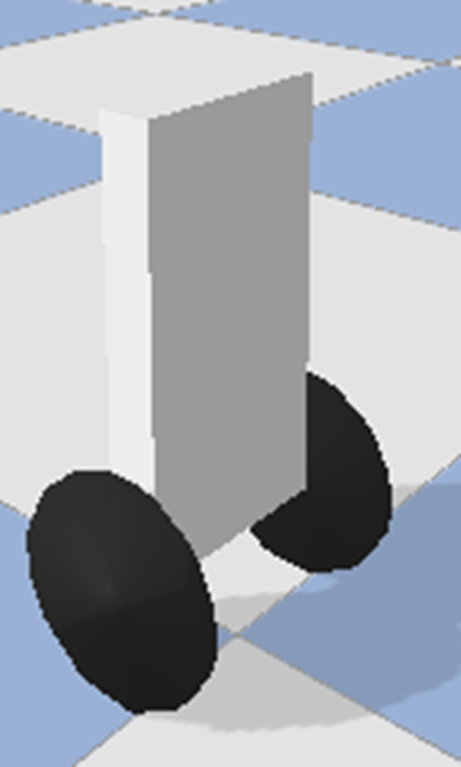
\includegraphics[width=\textwidth]{robot.png}
        \caption{The custom two-wheeled robot model.}
        \label{fig:robot_model}
    \end{minipage}\hfill
    \begin{minipage}{0.65\textwidth}
        \centering
        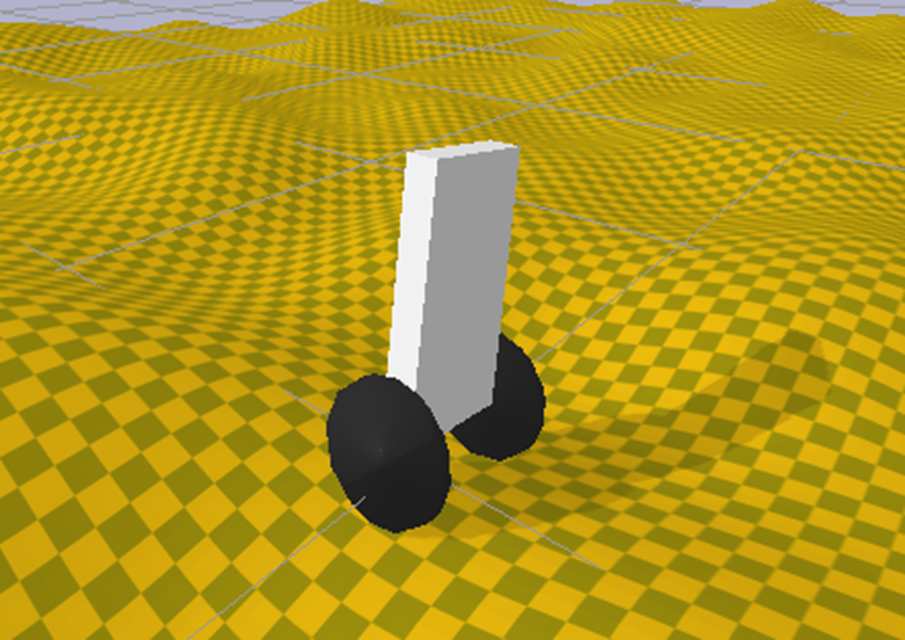
\includegraphics[width=\textwidth]{terrain.png}
        \caption{The uneven terrain used for testing.}
        \label{fig:uneven_terrain}
    \end{minipage}
\end{figure}


\subsection{PID Controller}
The PID controller was implemented to maintain the robot's balance by controlling its pitch and yaw, ensuring the robot stands upright. The controller operates in three modes: proportional, integral, and derivative, each contributing to the overall control strategy. The proportional mode ($K_p$) provides an immediate response to errors by applying a corrective force proportional to the current pitch error, helping the robot return to an upright position. The integral mode ($K_i$) addresses accumulated errors over time, ensuring that any persistent tilt is corrected by integrating past errors and applying a cumulative adjustment. The derivative mode ($K_d$) predicts future errors based on the rate of change of the pitch, allowing the controller to dampen oscillations and prevent overshooting by applying a force that counteracts rapid changes. The gains ($K_p$, $K_d$, $K_i$) were tuned iteratively, starting with $K_p$ to achieve basic stability, followed by $K_d$ and $K_i$ to reduce oscillations and ensure smooth balancing. The following code snippet illustrates the implementation of the PID controller:

\begin{verbatim}
def pid_control(error, prev_error, integral, dt):
    Kp = 1.0  # Proportional gain
    Ki = 0.1  # Integral gain
    Kd = 0.05 # Derivative gain

    # Proportional term
    P = Kp * error

    # Integral term
    integral += error * dt
    I = Ki * integral

    # Derivative term
    derivative = (error - prev_error) / dt
    D = Kd * derivative

    # PID output
    output = P + I + D
    return output, integral
\end{verbatim}

\subsection{Keyboard Navigation}
A manual navigation interface was implemented, allowing users to provide commands via the keyboard. These inputs were translated into force and yaw adjustments, enabling the robot to navigate both flat and uneven terrains.

\subsection{Autonomous Navigation}
In my exploration of reinforcement learning techniques for autonomous navigation, I experimented with three algorithms: Proximal Policy Optimization (PPO), Advantage Actor-Critic (A2C), and Deep Q-Network (DQN). Each algorithm was tested to determine its effectiveness in controlling the robot's force and yaw to reach predefined destinations on uneven terrain.

Initially, DQN was considered due to its simplicity and effectiveness in discrete action spaces. However, it struggled with the continuous control required for our robot, leading to suboptimal performance. A2C, with its actor-critic architecture, showed improvements over DQN by providing more stable learning through parallel environments. Despite this, A2C's performance was inconsistent, particularly in handling the complex dynamics of uneven terrain.

PPO emerged as the most promising algorithm, offering a balance between exploration and exploitation through its clipped objective function. It consistently outperformed both DQN and A2C in my tests, demonstrating superior stability and convergence rates. The success of PPO can be attributed to its ability to handle the continuous action space more effectively, which is crucial for the precise control needed in our application.

Hyperparameter tuning played a critical role in optimizing PPO's performance. I experimented with various learning rates, batch sizes, and discount factors to enhance the training process. The learning rate was fine-tuned to ensure efficient learning without overshooting, while the batch size was adjusted to balance computational efficiency and learning stability. Additionally, the discount factor was optimized to appropriately weigh future rewards, which is essential for long-term planning in navigation tasks.

Despite the advantages of PPO, training the model to navigate uneven terrain remained challenging due to the increased complexity of the environment. This complexity necessitated further refinement of the RL training pipeline to improve the model's robustness and adaptability.

\section{Contribution}
The key contributions of this project include:
\begin{itemize}
    \item Development of a custom robot model and terrain in PyBullet.
    \item Implementation of a PID controller for real-time stabilization.
    \item Integration of PPO for autonomous navigation.
    \item Insights into the challenges of RL in complex terrains.
\end{itemize}

\section{Results}
The \textit{BalanceBot} successfully balances and navigates flat terrain using both manual and autonomous control. On uneven terrain, manual keyboard navigation is functional, but the RL model struggled to achieve reliable autonomous navigation due to insufficient training data and complexity of the environment. These findings highlight the need for further refinement of the RL training pipeline.

\section{Conclusion}
This project demonstrates the feasibility of balancing and navigating a two-wheeled robot using PID and RL techniques. While the RL model faced limitations in uneven terrain, the robot's performance on flat surfaces and its manual operability on complex terrain underscore the potential for future improvements. Future work will focus on enhancing the RL model's robustness and exploring hybrid control strategies.

\section*{References}
\begin{thebibliography}{1}
\bibitem{schulman2017proximal} J. Schulman, F. Wolski, P. Dhariwal, A. Radford, and O. Klimov, "Proximal policy optimization algorithms," \textit{arXiv preprint arXiv:1707.06347}, 2017.

\bibitem{backyard} Backyard Robotics, "Build a balancing bot with OpenAI Gym: Part I," [Online]. Available: https://backyardrobotics.com.
\end{thebibliography}

\end{document}
